\documentclass[10pt,twoside]{article}


\usepackage[swedish]{babel}


\usepackage{color}
\PassOptionsToPackage{cmyk}{xcolor} % Makes sure that the active colour space is CMYK
\usepackage{pst-all}

\usepackage{ebgaramond}
\usepackage{array, booktabs}
\usepackage{rotating}
%\usepackage[x11names]{xcolor}
\usepackage{colortbl}
\usepackage{caption}
\usepackage{pdfpages}
\DeclareCaptionFont{blue}{\color{LightSteelBlue3}}


\usepackage{lettrine}

\usepackage{multicol}
\usepackage{enumitem}

\usepackage{lipsum}

\usepackage[absolute]{textpos}

\let\clipbox\relax

\usepackage{graphicx}
\usepackage{adjustbox}

\usepackage{xstring}
\usepackage{needspace}
\usepackage{changepage}

\usepackage{wrapfig}

\usepackage{tikz}
\usetikzlibrary{arrows,calc}

\usepackage{fotpackage}
\fotfil{AndraTexter/fotfil.txt}

\usepackage{inputsongpackage}
\usepackage{inputsongpackage2col}


\usepackage{multicol}
\usepackage{amssymb}
\usepackage{moresize}
\usepackage{paracol}

\usepackage{pgfplots}
\usepackage{amsmath}


\usepackage{watermark}
\usepackage{adjustbox}

\headheight=0pt
\headsep=0pt


\newlength\bleed
\setlength{\bleed}{0.5cm}

\newlength\AFiveWidth
\setlength{\AFiveWidth}{14.8cm}

\newlength\AFiveHeight
\setlength{\AFiveHeight}{21cm}

\usepackage[paperwidth=15.8cm,%=\AFiveWidth+2*\bleed %The size of the document, this allows for cropping to the actual document size determined by layoutwidth and layoutheight below
            paperheight=22cm,
            layoutwidth=14.8cm, %The width the printed materal will have. Setting this to exactly A5 width will risk that some cuts will be off and we'll get white edges around the front and back page. Thus TT recommends setting this to include bleed, i.e. the same as paperwidth above. Same argument goes for layoutheight below.
            layoutheight=21cm, %A5-paper height
            layouthoffset=0.5cm,
            layoutvoffset=0.75cm,
            top=1.5cm,
            bottom=3cm,
            left=1.75cm,
            right=1.75cm,
            %marginparwidth=4cm,
            %marginparsep=0.4cm
            ]{geometry}% För att fixa bleed-marginaler (mer info, via exempel, här: https://3d.bk.tudelft.nl/ken/en/2016/03/20/self-publishing-your-latex-thesis.html )


\parindent=0pt
\parskip=0pt



\newcommand{\Bilder}[1]{\begin{center}\includegraphics[width = 0.9\textwidth]{#1}\end{center}}


%\foto{bildadress j{\"a}mf{\"o}rt med main.tex}{Namn}{Post}
\newcommand\foto[3]{%
\begin{minipage}[t]{0.24\textwidth}
\parbox[c][3.2cm][c]{\textwidth}{\centering\adjincludegraphics[height=3.2cm]{#1}}\\[5pt]
\parbox[c][2.1\baselineskip][c]{\textwidth}{\centering\bf\small#2}\\[3pt]
%\raggedright #3
\centering\footnotesize #3
\vspace{0.7\baselineskip}
\end{minipage}\hfil%
}


\newcommand\openquote{
	\tikz[overlay,xshift=-15pt,yshift=0pt]
		\node {\fontsize{40}{40}\selectfont\bf``};
	\kern0pt
}
\newcommand\closequote{
	\tikz[overlay,anchor=north,xshift=15pt,yshift=0pt]
		\node {\fontsize{40}{40}\selectfont\bf''};
}

\newcommand\funnyquote[1]{
\begin{quote}
\openquote
{\large\bf#1}\hfill
\raisebox{\baselineskip}[0pt]{\closequote}
\end{quote}
}

\newcommand{\citat}[1]{“#1”}

\newcommand{\rubrik}[1]{{\begin{center}\Huge\sc#1\end{center}}\par}

\newcommand{\underrubrik}[1]{{\begin{center}\huge\sc#1\end{center}}\par}

\newcommand{\inlinerubrik}[1]{\large{\sc#1}}

% \newlength\watermarkbleed
\watermarkbleed=0.1cm
\newlength\watermarkxoffset
\newlength\watermarkyoffset
\newlength\watermarkwidth
\newlength\watermarkheight
\watermarkxoffset=\dimexpr -1.75cm-\watermarkbleed
\watermarkyoffset=\dimexpr 1.5cm-\paperheight-\watermarkbleed
\watermarkwidth=\dimexpr \paperwidth+2\watermarkbleed
\watermarkheight=\dimexpr \paperheight+2\watermarkbleed
\leftwatermark{\def\unitlength{}\put(\watermarkxoffset,\watermarkyoffset){\includegraphics[width=\watermarkwidth,height=\watermarkheight]{../Bilder/background_l3.png}}}
\rightwatermark{\def\unitlength{}\put(\watermarkxoffset,\watermarkyoffset){\includegraphics[width=\watermarkwidth,height=\watermarkheight]{../Bilder/background_r3.png}}}  % Settings for watermarks. Currently not used


\begin{document}


\pagestyle{empty}
%\pagenumbering{gobble}

%%% Framsida
%\thiswatermark{}
\includepdf[width = 158mm]{Bilder/OmslagFram.pdf} %15.8cm bred
\pagestyle{fotfil}
%\pagenumbering{arabic}

%%% Karakt{\"a}rsbeskrivningar	1
%%\thiswatermark{}
\begingroup
\newcommand\blockA[1]{\parbox[c][0.23\textheight][c]{0.3\textwidth}{\centering #1}}
\newcommand\blockB[1]{\parbox[c][0.23\textheight][c]{0.65\textwidth}{\raggedright #1}}

% Johannes Kepler
\blockA{\adjincludegraphics[height=0.27\textheight]{Bilder/Karaktarer/Einstein.png}}
\blockB{\textsc{Albert Einstein}\\
%Johannes är en ung astronom som spenderat sina dagar vid universitetet i Tübingen under skolning av Michael Mästlin. Han beundrar sin mentor Michael och vill göra honom stolt, men samtidigt stå på egna fötter. Han vill lära sig allt om allt och strävar efter att utveckla den vetenskap han älskar mest; astronomi.}
Albert Einstein i egen kort person. På senare år har den excentriska vetenskapsmannen dragit sig tillbaka från omvärldens rampljus för att ägna sig åt än mer excentriska idéer och uppfinningar. Om det är något som han har lärt sig under sitt långa liv är det att han alltid vet bäst, oavsett om han faktiskt har rätt eller inte. Alla hans resonemang är fullt underbyggda av logik och fysik medan andras åsikter och rimlighet spelar en mindre roll i tankeprocessen.}

% Michael Mästlin
\vfil
\blockB{\vspace{2ex}\textsc{Karl ``Kalle´´ Andersson}\\
%Michael är en bitter gammal gubbe med sin storhetstid bakom sig. Han har jobbat i många år vid universitet i Tübingen, men har nu fått en chans att hjälpa sin protogé, Johannes Kepler, uppåt i världen; och detta tänker han inte gå miste om. Han känner sedan tidigare Tycho och de har haft sina meningsskillnader, då han anser att Tychos mätningar inte står en chans mot hans teoretiska modeller.}
Kalle är Einsteins kollega samt en ung och lovande forskare med skarp blick och engagemang. Har han något som han vill säga drar han sig inte en sekund för att göra sin röst hörd -- om Einstein lyssnar på honom är dock en annan fråga. Kalle är en självsäker individ som vet vad han vill, såväl i forskning som i kärlek.}
\blockA{\adjincludegraphics[height=0.27\textheight]{Bilder/Karaktarer/Kalle.png}} \\ \\

%% Tycho Brahe
\vfil
\blockA{\adjincludegraphics[height=0.27\textheight]{Bilder/Karaktarer/Laplace.png}}
\blockB{\vspace{1ex}\textsc{Laplace}\\
Laplace är tvillingbror till Nabla och lite av en ensamvarg. Han brukar hänga vid sin verkstad och laga saker i lugn och ro, helst utan att prata för mycket med främlingar, men när tidsresenärer dyker upp är det svårt att inte vara nyfiken. Särskilt  när en av dem är så snygg och charmig (och nej, det är inte Einstein som avses). Nämnde vi förresten att han är en cyborg?}
%Tycho är en glad men utarbetad man på ålderns höst. Som långvarig hovastronom vet han var saker och planeter hör hemma och har inte tid för nymodigheter som heliocentrismen. Han störs ofta i sitt arbete av kejsaren som bryr sig mer om astrologi än astronomi!}

%% Rudolf II von Habsburg
\vfil
%\blockB{\textsc{Rudolf II von Habsburg} \\
%Rudolf är kejsare över det Tysk-Romerska riket och sitter på sin tron i det kejserliga palatset i Prag. Rudolf omger sig av vetenskapsmän och konstnärer, där hans favorit är hans bästa vän Giuseppe, och hade helst lämnat de tråkiga sakerna, som att styra riket, till andra och låter hellre ödet avgöra vad han ska göra. Han gillar konst och vetenskap, men han förstår sig inte på det själv.}
%Rudolf är kejsare över det Tysk-Romerska riket och sitter på sin tron i det kejserliga palatset i Prag. Rudolf omger sig av vetenskapsmän och konstnärer, där hans favorit är hans bästa vän Giuseppe, och hade helst lämnat de tråkiga sakerna, som att styra riket, till andra och låter hellre ödet avgöra vad han ska göra. Han gillar konst och vetenskap, men han förstår sig inte på det själv.}
%\blockA{\adjincludegraphics[height=0.27\textheight]{Bilder/Karaktarer/Rudolf.png}}


\endgroup

\newpage
\begin{center}

\rule{\textwidth}{1pt}
\rule{\textwidth-1cm}{0.4pt}\\
\vspace{0.3cm}
\textsc{\HUGE F-spexet 2022}\\
%\vspace{0.025\textheight}
\rule{0.3\textwidth}{0.4pt}\\
\vspace{0.025\textheight}
\textsc{\HUGE Tillbaka till dåtiden}\\
\vspace{0.2cm}
\textsc{\large eller}\\
\vspace{0.005\textheight}
\textit{\LARGE Einsteins äventyr i rumtiden}\\
\vspace{0.010\textheight}
\textsc{\normalsize eller}\\
\vspace{0.005\textheight}
\textit{\Large Albert the Explorer}\\
\vspace{0.0075\textheight}
\textsc{\small eller}\\
\vspace{0.0025\textheight}
\textit{\large Konsten att bibehålla en konstant rumtid}\\
\vspace{0.005\textheight}
\textsc{\footnotesize eller}\\
\textit{\normalsize Cyberpunk 2052}\\
\vspace{0.0025\textheight}
\textsc{\tiny eller}\\
\textit{\small Frågan är inte \emph{var} vi parkerade tidsmaskinen, utan \emph{när} vi parkerade tidsmaskinen}\\
\hrulefill\\
\vspace{\fill}
\parbox[c][][c]{0.45\textwidth}{\centering 
\includegraphics[width=0.35\textwidth]{Bilder/TidigareSpexloggor/2022Datiden.png}}
\parbox[c][][c]{0.45\textwidth}{\centering 
\includegraphics[width=0.33\textwidth]{Bilder/Loggor/Spexloggaoifylld3.png} \\\vspace{0.2cm}

\includegraphics[width=0.27\textwidth]{Bilder/Loggor/studieframjandet_samarbete.jpg}}


% \adjincludegraphics[width=0.3\textwidth]{Bilder/Loggor/Spexloggaoifylld3.png}
% \hspace{0.03\textwidth}
% \adjincludegraphics[width=0.3\textwidth]{Bilder/TidigareSpexloggor/2022Datiden.png}
% \hspace{0.03\textwidth}
% \adjincludegraphics[width=0.3\textwidth]{Bilder/Loggor/studieframjandet_samarbete.jpg}
\rule{\textwidth}{1pt}
\end{center}

\newpage

\vspace*{\fill}
\begingroup
\raggedright{
\huge{“En lycklig man är för nöjd med nuet för att vistas för mycket i framtiden” \\}
}
\endgroup
\begingroup
\begin{centering}
\huge{\ \\
\emph{\hspace{65mm} -- Albert Einstein}}
\end{centering}
\endgroup
\vspace*{\fill}
\newpage
%\null
\newpage


%%% V{\"a}lkommen
\rubrik{\huge\sc Några ord från styret}% \linebreak[1] eller nåt}
\begingroup
\fontsize{12}{12}\selectfont
\parskip=\baselineskip
\vspace{-0.5cm}\centering\large{\textit{\textsc{\textsw{ Varmt välkomna till F-spexet Tillbaka till Dåtiden!}}}}
\begin{adjustwidth}{23pt}{23pt}
Är er vardag trist och grå? Undrar ni vad framtiden har att erbjuda? Följ med oss på en spännande resa till år 2052! Albert Einstein har byggt en tidsmaskin tillsammans med sin kollega Karl Andersson och de reser 100 år fram i tiden för att lära sig om framtiden (och kanske hitta kärlek). Men när tidsmaskinen börjar att krångla behöver de all hjälp de kan få för att hitta sin väg tillbaka till dåtiden och förhindra rumtidens kollaps.

Det blir en kväll fylld av vetenskap, kärlek, en eller annan kupp samt väldigt många utklädnader och hattar. För att genomföra detta är vi en förening med ett 30-tal spexare som har arbetat med uppsättningen under året. Vi har övat teater och musik, målat kulisser och byggt rekvisita, sytt kläder, planerat och strukturerat, och mycket annat. Och naturligtvis även haft det riktigt roligt tillsammans! Vi hoppas att ni kommer få det minst lika roligt ikväll! Om ni vill veta mer om vilka vi är, titta längre bak i detta program.

Om du känner att det här med spex verkar vara kul och känner att du skulle vilja vara med nästa gång så rekommenderar vi att du fyller i vår asplapp som du finner senare i det här programmet och lämnar till närmsta spexare. Om du har några funderingar eller frågor kan du också alltid maila styret@f-spexet.se. Men nu ska vi inte uppehålla er längre, utan istället önska er en trevlig kväll och låta er återgå till er middag, föreställningen eller resten av programmet!

\begin{flushright}
\textit{\textsc{\textsw{Styret i F-spexet 2022}}}
\end{flushright}
\end{adjustwidth}

\endgroup

\newpage


%%% Meny


\begingroup
\rubrik{\Huge\sc Kvällens meny}
\begin{center}

\vfil

\newcommand\blockA[1]{\parbox[c][0.23\textheight][c]{0.4\textwidth}{\centering #1}}
\newcommand\blockB[1]{\parbox[c][0.23\textheight][c]{0.6\textwidth}{\raggedright #1}}

\LARGE\textsc{\textsw{Förrätt}}\\
\large\textsc{Rödbetscarpaccio}\\
\normalsize\textit{Tunt skivade rödbetor med bland annat sallad på. Den serveras kall, så den är perfekt för dig som inte kan styra din tidsmaskin rätt till servering.}

\vfill

\LARGE\textsc{\textsw{Huvudrätt}}\\
\large\textsc{Fransk potatissallad med kyckling och salsa}\\ 
\normalsize\textit{Utöver att resa i tiden kan tidsmaskinen IKAE även resa i rummet. Därför får ni nu en fransk potatissallad med kyckling och salsa.}

\vfill

\LARGE\textsc{\textsw{Efterrätt}}\\
\large\textsc{Chokladmousse}\\ 
\normalsize\textit{Så god att du önskar att du hade en tidsmaskin så att du kunde åka tillbaka i tiden efteråt för att få en portion till.}
\vspace{\fill}

\adjincludegraphics[width=0.2\textheight]{Bilder/Mat/rodbetor.jpg}
\hspace*{\fill}
\adjincludegraphics[width=0.2\textheight]{Bilder/Mat/franskpotatissallad.jpg}
\hspace*{\fill}
\adjincludegraphics[width=0.2\textheight]{Bilder/Mat/chokladmousse.jpg}

\end{center}
\endgroup



\newpage
\rubrik{årets rebus}

\hfill

Här hittar ni årets rebus. Fundera gärna under kvällen om ni kan lösa den!

\vspace{9pt}

Grattis till Anna och Elsa Ryberg, Elina Ryding, Sofia Damne och Viktor Rehnberg som löste rebusen i vår rebustävling!

\hfill
\begin{figure}[hbt!]
    \centering
    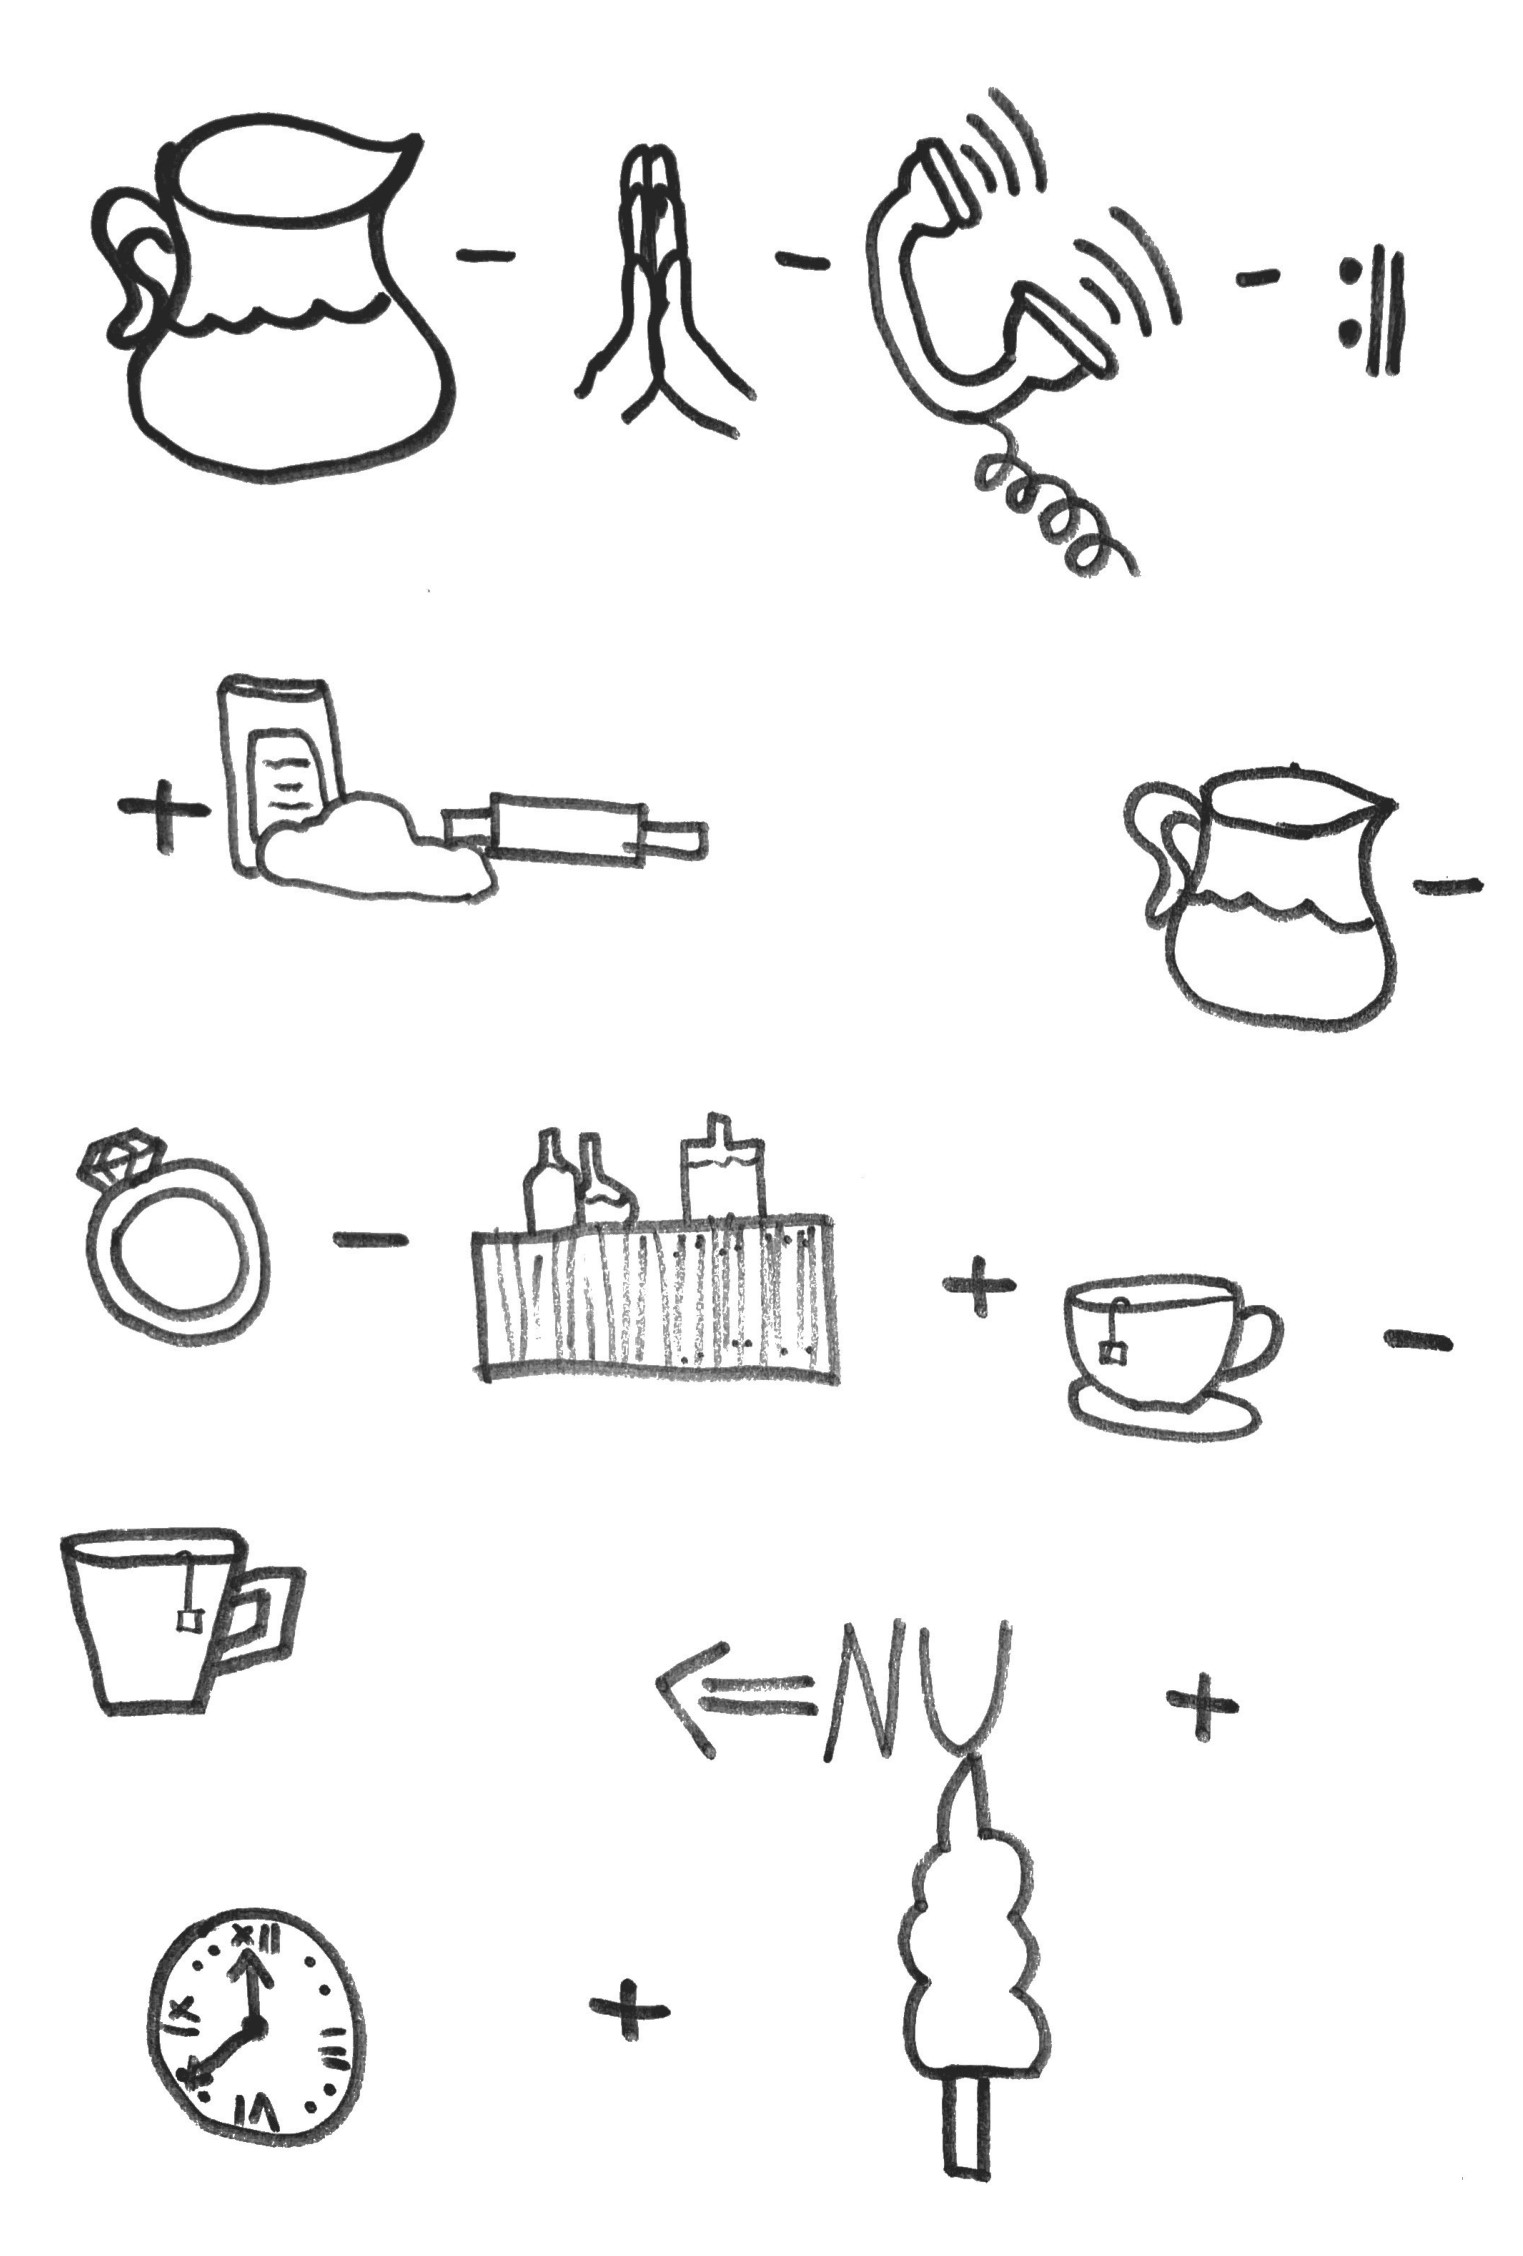
\includegraphics[width=0.5\textwidth]{Bilder/Rebus/Rebus-2022.jpg}
    \label{fig:my_label}
\end{figure}


\vfil

\underrubrik{Lösning på rebus (spoiler!)}

\begin{flushright}

\begin{turn}{180}
och en \textit{en}, alltså \textsc{dåtiden}. Då har vi årets tema: \textsc{Tillbaka till dåtiden}!
\end{turn}

\begin{turn}{180}
Sedan ser vi \textit{nu} med en pil bakåt vilket blir \textit{då}, och så lägger vi till \textit{tid} 
\end{turn}

\begin{turn}{180}
för att sedan lägga till \textit{t(e)} och ta bort \textit{te}. Då har vi fått ordet \textsc{till}.
\end{turn}

\begin{turn}{180}
Efter detta ser vi en ny \textit{tillbringare}. Även där tar vi bort \textit{ring} och \textit{bar} 
\end{turn}

\begin{turn}{180}
 vilket ger \textit{till}. Sedan lägger vi till \textit{baka} och får \textsc{Tillbaka}. 
\end{turn}

\begin{turn}{180} 
Vi ser en \textit{tillbringare} där vi sedan tar bort \textit{be}, \textit{ring} och \textit{re }för repristecknet,
\end{turn}

\end{flushright}



%%% Akt 1
\newpage
\pagestyle{fotfil}
\rubrik{\Huge\sc Akt i}
\vspace*{\fill}
\rubrik{Aktintro: \linebreak[1] \textbf{Tid-och-rumsförlagt-intro}}
\begin{center}{\large Arrangör: \textbf{Erik Karlsson Nordling och Pontus Nilsson}}\end{center}
\vfill
\begin{center}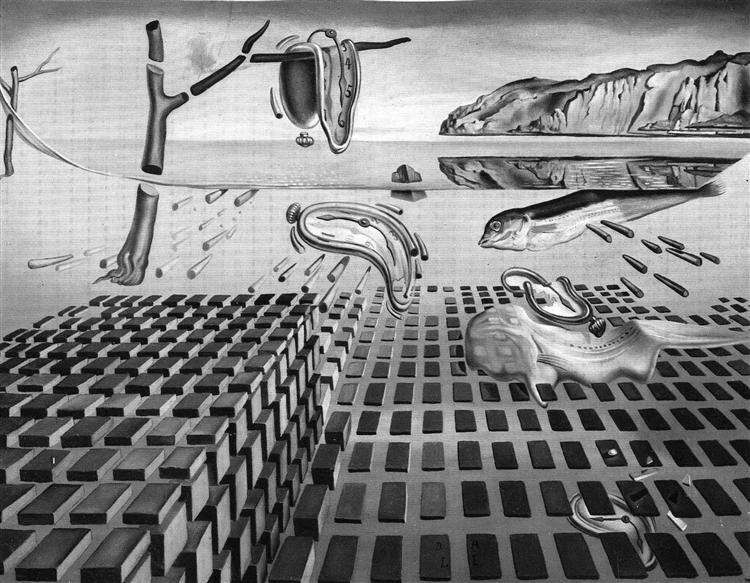
\includegraphics[width = 1\textwidth]{Bilder/Aktintron/Dali.jpg}
\end{center}
\newpage
\begingroup\fontsize{11}{12}\selectfont %\fontsize{<fontsize>}{<line spacing>}
\multicolinputsong{Akt1/kuplett_1_1_1.txt}
%\inputsong{Akt1/kuplett_1_1_1.txt}
\endgroup
\newpage
\begingroup\fontsize{11}{12}\selectfont
%\multicolinputsong{Akt1/kuplett_1_2_1.txt}
\inputsong{Akt1/kuplett_1_2_1.txt}
\endgroup
\newpage
\begingroup\fontsize{11}{12}\selectfont
\multicolinputsong{Akt1/kuplett_1_3_1.txt}
%\inputsong{Akt1/kuplett_1_3_1.txt}
\endgroup

\newpage


%%% Inrop
\underrubrik{Vi vill att du p{\aa}verkar vad som h{\"a}nder p{\aa} scen!}
\begingroup
\fontsize{11}{13}\selectfont
\parskip=0.5\baselineskip
G{\"o}r inrop!
I F-spexet {\"a}r det publiken som best{\"a}mmer genom att ropa hur skådespelarna ska agera. Har du en kul id{\'e} s{\aa} tveka inte att ropa till skådespelarna!

\underrubrik{Inropsbingo}
Om du vill ha lite mer utmaning kan du spela inropsbingo med en kompis. 
Innan f{\"o}rest{\"a}llningen b{\"o}rjar byter ni program med varandra och fyller i varandras spelplan, ett rop per ruta. Kom ih{\aa}g att s{\"a}ga ett pris ocks{\aa}, till exempel vem som skall k{\"o}pa l{\"a}sk i aktpausen.

N{\"a}r f{\"o}rest{\"a}llningen v{\"a}l har b{\"o}rjat kan ni eller andra i lokalen ropa och det {\"a}r till{\aa}tet att ropa saker fr{\aa}n sin egen bricka.  Om n{\aa}gon (t ex du) ropar det som st{\aa}r p{\aa} din bricka, och skådespelarna reagerar, s{\aa} kan den rutan p{\aa} brickan kryssas av. F{\"o}rst till 5 i rad ropar naturligtvis \citat{bingo}!

%\begin{multicols}{2}
%\begin{itemize}[labelwidth=7pt,leftmargin=!]\raggedright
%\item H{\"o}gre!
%\item H{\aa}rdare!
%\item Starkare!
%\item Mer psykedeliskt!
%\item Byt dialekt!
%\item Blygare!
%\item Som Kungen!
%\item Som en person som gjort bort sig!
%\item Varmare!
%\item Manligare/kvinnligare!
%\item Prata bakl{\"a}nges!
%\item Byt roller!
%\item Som en chalmersprofessor!
%\item Mer ordvitsar!
%\item Galnare!
%\item D{\"o}dare!
%\item P{\aa} norska!
%\item I falsett!
%\end{itemize}
%\end{multicols}
%
%

%\rubrik{Hur du f{\aa}r mer kupletter!}
%\lettrine[lines=3]{N}{{\"a}r} du minst anar det kommer folk p{\aa} scen bryta ut i s{\aa}ng till orkesterns ljuva ljud. 
%Om du tycker om kupletten kan du klappa ivrigt f{\"o}r att uppmuntra spexarna att framf{\"o}ra ytterligare en kuplett. 
%Om du tycker att kupletten var lite s{\aa} d{\"a}r, uppmuntra dem {\"a}nnu mer, s{\aa} kommer de framf{\"o}ra en ny version som ni tycker b{\"a}ttre om.
\begingroup\fontsize{10}{12}\selectfont


\begin{center}
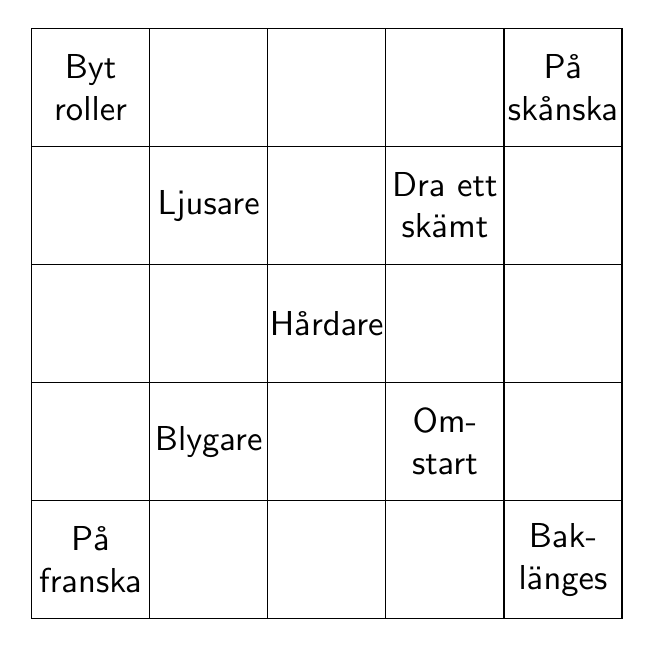
\begin{tikzpicture}[>=latex]
\tikzstyle{every node}=[font=\sf,align=center,scale=1.25]
\draw[step=1.5cm,color=black] (0,0) grid (7.5,7.5);
\node at (6.75,0.75) {Bak-\\l{\"a}nges};
\node at (5.25,2.25) {Om-\\start};
\node at (2.25,5.25) {Ljusare};
\node at (0.75,6.75) {Byt\\ roller};
\node at (6.75,6.75) {P{\aa} \\ sk{\aa}nska};
\node at (5.25,5.25) {Dra ett \\ sk{\"a}mt};
\node at (3.75,3.75) {H{\aa}rdare};
\node at (2.25,2.25) {Blygare};
\node at (0.75,0.75) {P{\aa}\\ franska};
\end{tikzpicture}
\end{center}

\endgroup
\endgroup


\newpage

\rubrik{Intresserad av F-spexet?
}
%\phantomsection\addcontentsline{toc}{section}{\sc Intresserad av F-spexet?\dotfill}
%\vspace{-cm}
%\begin{table}
\label{asplapp}

Det finns en massa roliga saker som man kan göra i F-spexet. Man kan stå på scen, bygga
rekvisita, laga mat, sköta hemsidan och mycket mer! \\

Här nedan finns mer utförliga beskrivningar av de olika posterna, så att du vet vad olika grupper har pysslat med under året. Här kan du också ta reda på vilken post som passar just dig, om du vill vara med i nästa års spex!\\

Vill du vara med? QR-koden nedan leder till vår digitala asplapp där ni kan hitta mer information och söka! %<Länk till aspformulär eller sidhänvisning> Mer information om aspningen finns \textbf{\textit{här}}.


\begin{center}
    
\includegraphics[width=0.3\textwidth]{Bilder/QR/F-spexet_aspformular.png}
\end{center}
\vspace{0.5cm}
\underrubrik{Grupper i F-spexet
}
\begingroup
\fontsize{11}{12}\selectfont
\parskip=1\baselineskip


{\Large\textit{Koreograf}} \\
När text och musik är fixat, behöver Skådespelarna en dans till dessa också, eftersom det blir lite tråkigt att titta på en person som står stilla och sjunger. Koreografen arbetar med att komma på danser som Skådespelarna ska framföra, och sedan lära Skådespelarna dessa. Detta innebär att ha extra mycket koll på sångerna och melodierna, samt att vara närvarande på Skådespelarnas rep lagom mycket.


{\Large\textit{Kostym}} \\
Det är Kostymgruppen som syr alla fina kläder på scen. Deras ansvar är att leta igenom manuset och bestämma hur Skådespelarna ska se ut, lista ut hur detta kan sys, sy det, och skälla när Skådespelarna har sönder sagda kläder. Ibland syr Kostym även viss tygbaserad rekvisita, exempelvis kuddar och draperier.

{\Large\textit{Kuplettsamordnare}} \\
För att spexet ska vara en musikal och inte bara en teater krävs det låtar och låttexter, i spexsammanhang kända som kupletter och kuplettexter. Kuplettsamordnaren ser till att kupletterna har vettiga och roliga melodier, att intresserade spexare skriver kuplettexterna, och att kupletterna blir färdiga i tillräckligt god tid för att Skådespelarna ska hinna lära sig dem.


{\Large\textit{Ljud och Ljus}} \\
LoL har till uppgift att bestämma vilken typ av ljud- och ljusutrustning årets spex behöver samt rigga denna innan föreställningarna. De fixar också ljudeffekter till spexet samt sköter reglagen under föreställningarna för att de som ska synas syns och de som ska höras hörs.


{\Large\textit{Manusförfattare}} \\
En av de mest essentiella ingredienserna för ett bra spex är ett bra manus. Manusgruppen är den grupp som innan andra spexare ens har kommit att tänka på nästa års spex redan har bestämt tema, synopsis, karaktärer, repliker, nödvändig rekvisita, lagt förslag på kupletter och en massa annat.

{\Large\textit{Mat}} \\
Matgruppen har som huvudsaklig uppgift att se till att det serveras en trerätters middag under föreställningarna. Detta innebär i realiteten att planera inköp, handla samt anpassa maten till olika allergier och matpreferenser. Förutom föreställningarna står Matgruppen även för maten på sittningar och dylikt inom spexet. Dessa processer förenklas något av att det finns spexare att tillgå under matlagningen som gör det faktiska hackandet, stekandet och kokandet enligt Matgruppens instruktioner.

{\Large\textit{Media}} \\
Mediagruppen ser till att folk vet vad spexet håller på med, ansvarar för all reklam såsom biljetter och affischer, gör programmet till föreställningarna, sköter spexets hemsida och sociala medier, samt dokumenterar såväl föreställningarna som arbetet under året. Media är lite av en paraply-grupp, så här passar många intressetyper in. Design, foto, film, kodande, PR, rebusskapande, skrivande och att beställa roliga saker från nätet är alla uppgifter som ryms inom Mediagruppen.

\newpage

{\Large\textit{MåBra}} \\
MåBra har till uppgift att övriga spexare (och de själva) mår bra, har det så roligt som möjligt och gör sitt bästa. För att uppnå sitt mål brukar de använda sig av ett hemligt vapen gemenligen kallat ``kakor”. MåBra-gruppen har ett antal fasta arbetsuppgifter: de sköter baren under föreställningarna, fixar pizza och liknande åt spexarna när spexet har jobbat hela dagen och fixar fika till vissa spexaktiviteter. Utöver detta kan de baka kakor, fixa peppiga spellistor, ha en massage-station... Det finns ingen gräns för hur bra spexarna kan må!


{\Large\textit{Orkester}} \\
Det är Orkestern som förgyller föreställningarna med fantastisk live-musik. Förutom att arrangera kupletter och spela upp dessa, spelar de också ett aktintro till varje akt. En bra färdighet i Orkestern är, förutom att så klart kunna spela sitt instrument, att arrangera musik. Orkestern repar vanligtvis mellan två och tre gånger i veckan.


{\Large\textit{Producent}} \\
Producenten är spexets allmänt konstnärliga ledare för hela föreställningen. Det innebär att producenten ser till att spexet har en enhetlig konstnärlig vision, och har på så sätt ett finger med i såväl rekvisita som kupletter, och samordnar mellan grupperna överlag.


{\Large\textit{Regissör}} \\
Regissörens uppgift är att leda Skådespelarnas rep, samt gnälla och tjata på Skådespelarna så att de gör rätt saker vid rätt tillfälle under dessa rep (naturligtvis med en grund i årets manus). Som Regissör är man också ansvarig för att det blir rep lagom ofta, både för Skådespelarna själva och tillsammans med Orkestern.


{\Large\textit{Scen}} \\
Varje spexmanus kräver en mängd dekor och rekvisita. Det kan var allt från böcker eller papper till nycklar och kanoner, lönndörrar, och diverse sorters maskiner. Scengruppen
behöver använda sin uppfinningsrikedom för att snickra, pyssla, bygga, och måla allt detta. Scengruppens ansvar är också att se till så att det existerar en faktisk scen att spela upp spexet på och kulisser att spela upp spexet framför. Under föreställningarna står Scengruppen redo att diskret ge rätt Skådespelare rätt sak vid rätt tillfälle, eller förflytta
rekvisita enligt manuset.

{\Large\textit{Skådespelare}} \\
Även kallad Ensemblen. Skådespelarnas uppgift i spexet är att stå på scen och framföra det spex som manusgruppen har drömt upp, regissören regisserat och publiken bett om. Den som blir invald som Skådespelare får en roll tilldelad sig, och sätter därefter igång med att lära sig manuset, sångtexter och dansstegen utantill. De övar också på improvisation inför inropen. Skådespelarna repar under ledning av Regissören, både på egen hand och tillsammans med Orkestern. Det brukar bli i genomsnitt tre kvällar i veckan under året.


{\Large\textit{Smink}} \\
Detta är gruppen som ger spexare färg och gör så att Skådespelarna ser ut som sina karaktärer med hjälp av peruker, smink, träben, huggtänder och dylikt. De flesta Skådespelare lär sig applicera rätt smink själva, men Sminkgruppen ska vara beredda på att få måla mycket i andras ansikten.

{\Large\textit{Styret}} \\
Styret är de som ansvarar för att det överhuvudtaget blir ett F-spex. De sitter i otaliga möten för att planera, boka, styra, och se till att spexet fungerar och är roligt. 
Ordföranden, som även går under namnet Tant, leder styrets arbete och är F-spexets ansikte utåt. 
Förmannen, vanligen kallad Fröken, är spexets arbetsledare som ser till att varje grupp arbetar och gör det de ska, samt planerar och leder spexets aktiviteter. 
Kassören, även kallad Fru, har ansvar för spexets ekonomi, och uppgifterna utgörs framförallt av att sköta bokföringen och ansvara för biljettförsäljningen. 
De övriga posterna är ledamöter. För alla stora och små uppgifter som inte täcks av de andra posterna finns det alltid en ledamot som kan ställa upp och föra spexets arbete framåt.


\endgroup
\newpage
\

\

%%% Akt 2
\rubrik{\Huge\sc Akt ii}
\vspace*{\fill}
\rubrik{Aktintro: \linebreak[1] \textbf{Folkmakt-intro}}
\begin{center}{\large Arrangör: \textbf{Ett ``demokratiskt'' intro skrivet av Orkestern och Arrare, a la ``viskleken'' style}}\end{center}
\begin{center}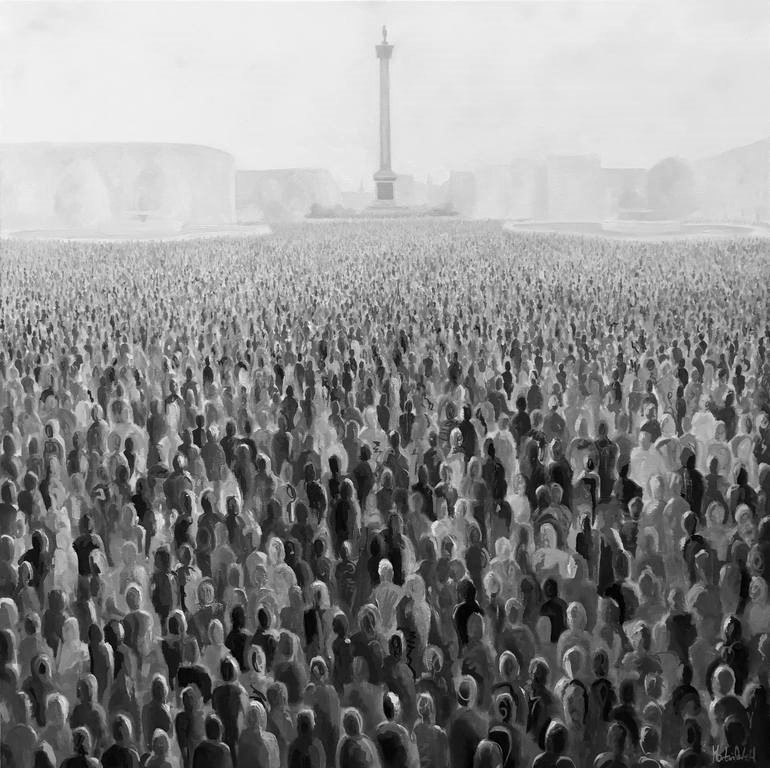
\includegraphics[width = 0.7\textwidth]{Bilder/Aktintron/crowd.jpg}
\end{center}

\vspace*{\fill}
\newpage
\begingroup\fontsize{11}{12}\selectfont %\fontsize{<fontsize>}{<line spacing>}
\multicolinputsong{Akt2/kuplett_2_1_1.txt}
%\inputsong{Akt2/kuplett_2_1_1.txt}
\endgroup
\newpage
\begingroup\fontsize{11}{12}\selectfont
\multicolinputsong{Akt2/kuplett_2_2_1.txt}
%\inputsong{Akt2/kuplett_2_2_1.txt}
\endgroup
\newpage
\begingroup\fontsize{11}{12}\selectfont
\inputsong{Akt2/kuplett_2_3_1.txt}
\endgroup
\newpage
\begingroup\fontsize{11}{12}\selectfont
\inputsong{Akt2/kuplett_2_4_1.txt}
\endgroup
\newpage



\newpage

%%% Tidslinje
\rubrik{\Huge\sc F-spexet vill tacka\dots
}
%\vspace{-cm}
%\begin{table}

\begin{center}

\includegraphics[width = 0.6\textwidth]{Bilder/Loggor/Flogga.png}
\end{center}

\begingroup
\fontsize{12}{13}\selectfont
\parskip=1\baselineskip

\begin{adjustwidth}{14pt}{14pt}
{\it Sök till Teknisk fysik!}


Våra studenter kännetecknas av sin problemlösningsförmåga, som i
kombination med den starka teoretiska grunden i matematik och fysik gör dem
attraktiva på arbetsmarknaden. I stort sett alla stora teknikföretag har
tekniska fysiker i personalstyrkan. Oftast hittar man dem på en forsknings-
eller utvecklingsavdelning och i ledande positioner. Teknisk fysik och
Teknisk matematik är de två mest teoretiska utbildningarna i Chalmers
programutbud. Du kommer helt enkelt att läsa matematik, fysik och teknik på
en hög och avancerad nivå.


{\it \dots Eller kanske Teknisk matematik?}


Studenter som väljer Teknisk matematik tycker att matematik är roligt,
utmanade och användbart. De uppskattar utbildningens teoretiska tyngd och
ser fram emot att lösa komplexa problem. Känner du igen dig i
beskrivningen? Under utbildningen får du en gedigen träning i
problemlösning och lär dig att använda kraftfulla matematiska verktyg, som
ger dig stora möjligheter till utmanande jobb i flera branscher.

%\begin{center}
%
\includegraphics[width = 0.6\textwidth]{Bilder/Loggor/Flogga.png}
%\end{center}
\end{adjustwidth}
\endgroup
\newpage


%%% Akt 3
\rubrik{\Huge\sc Akt iii}
\vspace*{\fill}
\rubrik{Aktintro: \linebreak[1] \textbf{Ikaros-intro}}
%\rubrik{Rysk promenad}
\begin{center}{\large Arrangör: \textbf{Viktor Skott och Gustav Axelsson}}\end{center}
% TODO bild
\begin{center}
\includegraphics[width = 0.7\textwidth]{Bilder/Aktintron/sol.jpg}
\end{center}

\vspace*{\fill}
\newpage
\begingroup\fontsize{11}{12}\selectfont %\fontsize{<fontsize>}{<line spacing>}
\inputsong{Akt3/kuplett_3_1_1.txt}
\endgroup
\newpage
\begingroup\fontsize{10}{12}\selectfont
%\multicolinputsong{Akt3/kuplett_3_2_1.txt}
\inputsong{Akt3/kuplett_3_2_1.txt}
\endgroup
\newpage
\begingroup\fontsize{11}{12}\selectfont
\inputsong{Akt3/kuplett_3_3_1.txt}
\endgroup

\newpage

%%% {\aa}rets spexare
%\rubrik{\Huge\sc Årets spexare}
%\vspace{0.5cm}
\rubrik{årets spexare}
\begin{center}
\foto{Bilder/spexare/__default_clock.jpg}{Spexare 1}{Grupp -- post}
\foto{Bilder/spexare/__default_clock.jpg}{Spexare 2}{Grupp -- post}
\foto{Bilder/spexare/__default_clock.jpg}{Spexare 3}{Grupp -- post}
\foto{Bilder/spexare/__default_clock.jpg}{Spexare 4}{Grupp -- post}\\
\foto{Bilder/spexare/__asp.jpg}{Du}{Asp}
\foto{Bilder/spexare/__gamle.jpg}{Den gamle}{Patet}

\end{center}

\vfill

%\newpage
%\rubrik{\Huge\sc Rita din egen stjärnbild!}
    \null
    \vfill
    \begin{tikzpicture}
        %\pgfmathsetseed{24122215}%This seed gave a butterfly shape
        \foreach \p in {1,...,100}
        { \fill (6*rand,6*rand) circle (0.05);
        }
    %\end{axis}
    \end{tikzpicture}
    \vspace*{\fill}
\newpage
%%% Gamla spex
\rubrik{Tidigare F-spex}
\newlength{\gamlaAffischerLength}
\setlength{\gamlaAffischerLength}{0.28\textwidth}
\newlength{\gamlaAffischerHeight}
\setlength{\gamlaAffischerHeight}{0.32\textwidth}
\vfill
\begin{tabular}{c c c}

\includegraphics[width=\gamlaAffischerLength]{Bilder/TidigareSpexloggor/BillyIcon} &

\includegraphics[width=\gamlaAffischerLength]{Bilder/TidigareSpexloggor/HeraIcon} &

\includegraphics[width=\gamlaAffischerLength]{Bilder/TidigareSpexloggor/AgathaIcon}\\


\includegraphics[height=\gamlaAffischerHeight]{Bilder/TidigareSpexloggor/BeowulfBra.jpg} &
%\adjincludegraphics[height=\gamlaAffischerHeight,clip=true,trim = 65 35 65 65]{Bilder/TidigareSpexloggor/Affisch_fantomen09.pdf} &

\includegraphics[width=\gamlaAffischerHeight]{Bilder/TidigareSpexloggor/Logga_fantomen} &

\includegraphics[height=\gamlaAffischerHeight]{Bilder/TidigareSpexloggor/Mary_logga.jpeg}\\


\includegraphics[width=\gamlaAffischerLength]{Bilder/TidigareSpexloggor/MediciIcon} &

\includegraphics[width=\gamlaAffischerLength]{Bilder/TidigareSpexloggor/ThorIcon}&

\includegraphics[width=\gamlaAffischerLength]{Bilder/TidigareSpexloggor/LudwigIcon} \\

\includegraphics[width=\gamlaAffischerLength]{Bilder/TidigareSpexloggor/KubaIcon}&

\includegraphics[width=\gamlaAffischerLength]{Bilder/TidigareSpexloggor/ZeldaIcon.png}&

\includegraphics[width=\gamlaAffischerLength]{Bilder/TidigareSpexloggor/UrIcon.png}
\\
\end{tabular}
\vfill
\newpage
\begin{tabular}{ccc}
    
\includegraphics[width=\gamlaAffischerLength]{Bilder/TidigareSpexloggor/jules_verne.png}&
    
\includegraphics[width=\gamlaAffischerLength]{Bilder/TidigareSpexloggor/CeciliaVasa.png}&
    
\includegraphics[width=\gamlaAffischerLength]{Bilder/TidigareSpexloggor/Doden.png}
\end{tabular}
\begin{center}
\begin{tabular}{cc}
    
    
\includegraphics[width=\gamlaAffischerLength]{Bilder/TidigareSpexloggor/logga_kepler.png}&
    
\includegraphics[width=\gamlaAffischerLength]{Bilder/TidigareSpexloggor/2021_Rockefeller.png}

%& \raisebox{14pt}{\includegraphics[width=\gamlaAffischerLength]{Bilder/TidigareSpexloggor/spexlogga_vit_591x567.png}}
\end{tabular}
\end{center}

\vfill
\underrubrik{Vill du inte missa något som händer?}
\vspace{0.3cm}
%\vspace{\fill}

\hspace{0.5cm}\adjincludegraphics[width=0.15\textheight]{Bilder/QR/F-spexet_facebook.png}
\hspace*{\fill}
\adjincludegraphics[width=0.15\textheight]{Bilder/QR/F-spexet_instagram.png}
\hspace*{\fill}
\adjincludegraphics[width=0.15\textheight]{Bilder/QR/F-spexet_hemsidan.png}\hspace*{0.5cm}\\
\hspace*{0.9cm}Facebook\hspace*{\fill} Instagram\hspace*{\fill} f-spexet.se\hspace{0.9cm}

\pagestyle{fotfil}

\newpage
\setlength{\columnsep}{0.6cm}
\setlength{\columnseprule}{0.2pt}
\begin{multicols}{2}
    {\centerline{\Huge \textsc{Aspa}}}\leavevmode\\
    \noindent F-spexet är en förening där det viktigaste är att ha kul. Tillsammans roar vi både oss själva och en hel del andra personer som råkar vara i närheten. Beroende på ditt specialintresse, månde det vara att sjunga, spela instrument, eller bara vara allmän pajas så hittar du din plats i vårt underbara spex.\leavevmode\\
    
    \noindent Är du sugen, men vet inte riktigt vad du kan hjälpa till med? Hugg tag i en spexare så berättar hen mer!\leavevmode\\
    
    \noindent Vill du komma och hjälpa till på en föreställning för att se hur det är? Hugg tag i en spexare så berättar hen mer!\leavevmode\\
    
    \noindent Vet du redan nu att du vill vara med i\break {F-spexet}? Riv av högersidan, fyll i, och lämna den till valfri spexare!

    \vspace*{\baselineskip}
    {\hfill }\vfill

    \centering
    
\includegraphics[width=\columnwidth]{Bilder/Loggor/Spexloggaoifylld3.png}
    
    \columnbreak
    
    {\centerline{\Huge \textsc{F-spexet}}}\leavevmode\\
    Jag är bra på att...
    \renewcommand\labelitemi{$\square$}
    \renewcommand\labelitemii{$\square$} 
    \footnotesize   
    \setlength{\columnsep}{0.1cm}
    \begin{multicols}{2}
        \begin{itemize}
            \setlength{\itemindent}{-1.5em}
            \setlength\itemsep{1pt}
            \item Banka
            \item Städa
            \item Sminka
            \item Göra reklam
            \item Designa
            \item Filma
            \item Fota
            \item Planera
            \item Improvisera
            \item Bokföra
            \item Regissera
            \item Spela\\ \hspace{-1.5em}instrument\\\hspace{-1.5em}\underline{\hspace{1.5cm}}
            \columnbreak
            \item Sjunga
            \item Dansa
            \item Baka
            \item Laga mat
            \item Kramas
            \item Blanda drinkar
            \item Koda
            \item Måla
            \item Skriva
            \item Tejpa
            \item Sy
            \item Beställa pizza
            \item \underline{\hspace{1.5cm}}
        \end{itemize}  
    \end{multicols}
    {\normalsize Jag vill söka posten...}
    \footnotesize
    \begin{multicols}{2}
        \begin{itemize}
        \setlength{\itemindent}{-1.4em}
        \setlength\itemsep{0.75pt}
            \item Ordförande
            \item Förman
            \item Kassör
            \item Ledamot
            \item Koreograf
            \item Regissör
            \item Producent            
            \item Kuplettarrare
            \item Kuplettsamordnare
            \item Kostym
            \item Ljud och Ljus
            \item Orkester,\\ \hspace{-1.5em}instrument:\\\hspace{-1.5em}\underline{\hspace{1.5cm}}
            \columnbreak
            \item Manusförfattare
            \item Mat
            \item MåBra
            \item Media:
            \vspace{-0.3pt}
            \begin{itemize}
                \setlength{\itemindent}{-3.2em}
                \setlength\itemsep{0.2pt}
                \item Hemsida
                \item Design
                \item PR
                \item Dokumentation
                \item Program
            \end{itemize}
            \item Scen
            \item Skådespelare
            \item Smink
            \item Annat: \\\hspace{-1.5em}\underline{\hspace{1.5cm}}
        \end{itemize}
    \end{multicols}
    \begin{itemize}
        \item Jag är F:are
        \item Jag kan tänka mig att ansvara för en grupp
    \end{itemize}
    \normalsize
    Namn:\underline{\hspace{4.62cm}}\\
    Email:\underline{\hspace{4.71cm}}\\
    Telefon:\underline{\hspace{4.471cm}}
\end{multicols}

\
\begin{paracol}{2}
    \vspace*{\baselineskip}
    {\hfill }\vfill{\noindent Här kan du rita en bild, eller skriva något, och lämna in!}
    
    \switchcolumn
    
    {\HUGE \textsc{Tack till}}
    \leavevmode\\
    
    \noindent\textbf{Fysikteknologsektionen}\\
    För att vi får bo hos er\leavevmode\\
    \vspace*{-0.3\baselineskip}

    \noindent\textbf{DP, F6, FnollK, F-styret}\\
    För Focus och allt annat\leavevmode\\
    \vspace*{-0.3\baselineskip}
    
    \noindent\textbf{Barocken}\\
    För det ovärderliga avtalet om Holt\leavevmode\\   \vspace*{-0.3\baselineskip}
    
    \noindent\textbf{Kulturkrock}\\
    För myggor och annat oknytt\leavevmode\\    \vspace*{-0.3\baselineskip}

    \noindent\textbf{LoB}\\
    För att vi syns och hörs\leavevmode\\    \vspace*{-0.3\baselineskip}

    \noindent\textbf{TecknologTryck}\\
    För program och manus\leavevmode\\    \vspace*{-0.3\baselineskip}

    \noindent\textbf{Jon och Roger}\\
    För lokalen KG\leavevmode\\    
    \vspace*{-0.3\baselineskip}

    \noindent\textbf{Chalmersspexet}\\
    För de trevliga utbytena\leavevmode\\     \vspace*{-0.3\baselineskip}

    \noindent\textbf{Alla som gav återkoppling på manus}\\
    För återkopplingen de gav på manus (duh!)\leavevmode\\    \vspace*{-0.3\baselineskip}

    \noindent\textbf{Studiefrämjandet}\\
    För all hjälp och kulissmålningslokalen\leavevmode\\    \vspace*{-0.3\baselineskip}

    \noindent\textbf{Julie Rowlett \& Jonathan Weidow}\\
    För bidrag och engagemang\leavevmode\\    \vspace*{-0.3\baselineskip}

    \noindent\textbf{Spidera}\\
    För att hemsidan fungerar\leavevmode\\    \vspace*{-0.3\baselineskip}

    \noindent\textbf{Carlsberg och QQ7}\\
    För backarna till scenen\leavevmode

\end{paracol}

\
\newpage

%\ \vfill Denna sida har avsiktligt l{\"a}mnats blank s{\aa} att ni ska kunna rita p{\aa} n{\aa}got mer permanent {\"a}n duken
%\newpage


%%% Karakt{\"a}rsbeskrivningar	2
%\thiswatermark{}
\begingroup
\newcommand\blockA[1]{\parbox[c][0.23\textheight][c]{0.3\textwidth}{\centering #1}}
\newcommand\blockB[1]{\parbox[c][0.23\textheight][c]{0.65\textwidth}{\raggedright #1}}

% Magdalene Brahe
\blockA{\adjincludegraphics[height=0.27\textheight]{Bilder/Karaktarer/Nabla.png}}
\blockB{\textsc{Nabla}\\
%Magdalene är dotter till Tycho och en baddare på mätteknik. Hon är glad och livlig men tar jobbet och studierna som astronom väldigt seriöst. Hon drömmer om kärlek, men självklart på sina egna villkor.}
Nabla är tvillingsyster till Laplace. Otrolig intelligens, övermänsklig charm, magnifik fysik. Alla dessa och fler är egenskaper som hon inbillar sig att hon besitter. Cybernetisk augmentation är hennes passion och hon missar aldrig en chans att förbättra sin kropp med ny teknik, vilket också är anledningen till att hon hjälper Mr. Andersson med hans forskning. Behöver kanske inte nämnas att hon också är en cyborg.}
% Giuseppe Arcimboldo
\vfil
\blockB{\vspace{2ex}\textsc{Mr. Andersson}\\
%Giuseppe är hovkonstnär vid det kejserliga hovet i Prag. Han är bekväm med sitt jobb, där han målar porträtt varje dag, och är bästa vän med kejsare Rudolf II. Han anser sig själv vara den bästa och vackraste konstnären i hela den vida världen, men hans konststil skulle kunna beskrivas som väldigt enkelspårad och enformig. Men självklart håller inte Giuseppe med om det, det finns ju ändå över 3000 olika päron.}
Mr. Andersson, den i framtiden välkända cybertroniska entreprenören. Ingen kan cyborger och biomekaniska implantat som han men det hindrar honom inte från att ständigt arbeta för att förbättra sina kreationer till den grad att han inte bryr sig om vad som är artigt eller moraliskt. Hans nästa idé är att använda rumtidsanomalier för att skapa implantat som är bättre än fysiskt möjligt. Att hitta en anomali är dock mycket svårt eftersom rumtiden är irriterande stabil och det är ju inte direkt så att det ofta sker händelser, typ tidsresor, som stör den. Eller?
}
\blockA{\adjincludegraphics[height=0.27\textheight]{Bilder/Karaktarer/Mr.Andersson.png}} \\ \\

%% Sofonisba Anguissola
\vfil
\blockA{\adjincludegraphics[height=0.27\textheight]{Bilder/Karaktarer/Lisa.png}}
\blockB{\vspace{1ex}\textsc{Lisa}\\
%Sofonisba är en ung men framstående konstnär från Cremona, Italien, som den senaste tiden jobbat för det spanska Hovet. Hennes jobb har blivit lovprisat av Michelangelo själv, men trots det så får hon inte så många möjligheter som konstnär. Hon har alltid svar på tal och hoppas att hon en dag ska få samma möjligheter som hennes manliga kollegor.}
Lisa är en otypisk framtidsmedborgare som arbetar hårt för att försörja sig. För att vara så effektiv som möjligt har Lisa flera olika jobb, men de olika yrkesuppgifterna är inget som gör henne förvirrad. Tvärtom går hon in i sina olika yrkesroller med total hängivelse. Kanske lite för total för att det ska vara psykiskt rimligt, även med framtida mått mätt.}

%% Hildegard
\vfil
%\blockB{\textsc{Hildegard} \\
%Hildegard är en tjänsteflicka vid det kejserliga hovet i Prag. Hon är medveten om alla intriger som sker på hovet, men vet samtidigt att det inte är hennes plats att lägga sig i det. Och även om hon gjorde det så är det ju inte precis någon som bryr sig om vad tjänstefolket tycker eller tänker.}
%Hildegard är en tjänsteflicka vid det kejserliga hovet i Prag. Detta innebär att hon kan allt om vad intriger heter, men inte kan göra något åt dem. Att ingen bryr sig om vad en säger tillåter en viss frispråkighet, vilket Hildegard utnyttjar fullt.}
%\blockA{\adjincludegraphics[height=0.27\textheight]{Bilder/Karaktarer/Hildegard.png}}


\endgroup

\newpage
\pagestyle{empty}


%%% Baksida
%\thiswatermark{}
\includepdf[width = 158mm]{Bilder/OmslagBak.pdf}
\end{document}
